
\documentclass[a4paper,english]{IEEEtran}
\usepackage[T1]{fontenc}
\usepackage[latin9]{inputenc}
\usepackage{graphicx}

\usepackage[unicode=true, pdfusetitle,
 bookmarks=true,bookmarksnumbered=false,bookmarksopen=false,
 breaklinks=false,pdfborder={0 0 1},backref=false,colorlinks=false]{hyperref}

\makeatother

\usepackage{babel}

\begin{document}

\date{December 2011}

\author{Alexandre Chappuis, Bastian Marquis and David Klopfenstein @ EPFL.ch}

\title{Implementation of a BGP Route Flap Damping Algorithm for the Bird
Routing Project}

\maketitle

\begin{abstract}
Today's Internet stability strongly relies on the good behaviour of
dynamic routing protocols such as BGP (Border Gateway Protocol), which
enables routing between Autonomous Systems. Route flapping is a well-known
and undesirable phenomenon occurring in both commercial and private
networks. In this report, we explain our implementation of the RFC
2439, BGP Route Flap Damping, for one famous Open Source routing software
suite, the Bird Routing Project.

We also present results of 3 experiments leading to a comparison on the impact that
BGP updates have in a network with and without route flap damping. The setup was
such that only one of the BGP routers was receiving updates from the external world.
\end{abstract}

\section{Introduction}

The inter-domain routing protocol BGP is still surviving to the gigantic
growth of the Internet that started during the last decade. However,
some widely used applications, such as Skype, still suffer from weaknesses
in that protocol. The main problems are twofold: firstly, BGP has
a slow convergence time, meaning that a change at one location can take
long before it is propagated to the other ends of the network.
Secondly, if a node becomes unstable, for example if its connectivity
constantly comes up and down, it will have bad consequences on the
network, both in terms of useless processing at BGP routers and unnecessary
routing traffic. Routes advertised and withdrawn at regular interval
of time are said to be \textit{flapping}.

Many approaches to counter route flapping were developed in
the late 90's. RFC 2439\cite{rfc2439} standardized one such approach:
it basically blocks updates from flapping routes, and does so until
the routes are deemed stable again. This RFC has been used extensively
for many years, in both commercial and open source routers.

Although this standard is not recommended any more\cite{ripe recommendations}
for today's routers, we wanted to implement it for the Bird Routing
Project\cite{bird}, hoping that it would serve as a good basis for
future possible improvements and extensions. There exist
many variants of the Route Flap Damping algorithm and the community
has not lost its interest in finding robust mechanisms that could
allow BGP to be more resilient.


\section{Overview}

RFC 2349 seeks to limit the impact of route flapping by ``damping''
(\textit{i.e.} ignoring packets of) misbehaving routes. The solution
must be able to distinguish flapping routes from good routes and consume
few resources, both in terms of memory usage and process time. The
RFC solves these problems by assigning each route a penalty term.
Whenever this penalty term for a given route reaches a certain threshold,
further advertisements for that route are ignored. This penalty term
varies over time : it is increased when the route becomes unreachable
and decays as long as the route stays stable. As soon as the figure
of merit goes below a \textit{reuse threshold}, the route can be used
again.

The figure of merits decays exponentially over time. Exponential decay
has several advantages : it can be implemented very efficiently using
precomputed \textit{decay arrays}. Also, with exponential decay, the
figure of merit keeps trace of previous instabilities for a fairly
long time : old instabilities become less and less important over
time, whereas fresh ones get penalized.

Network administrators have lots of freedom in choosing the behaviour
of the penalty term : they can control the half-life of the penalty
term, the maximum time interval a route can be suppressed (thus 
controlling the maximum penalty) and both the reuse and cut thresholds.

Figure \ref{fig_penalty} is an example of how the figure of merit 
evolves over time (the illustration comes from \cite{damping-pic}).
The route flaps three times, exceeding the cut threshold only after 
the third flap. The route is reused as soon as its penalty term goes 
below the reuse limit.

\begin{figure}
\begin{center}
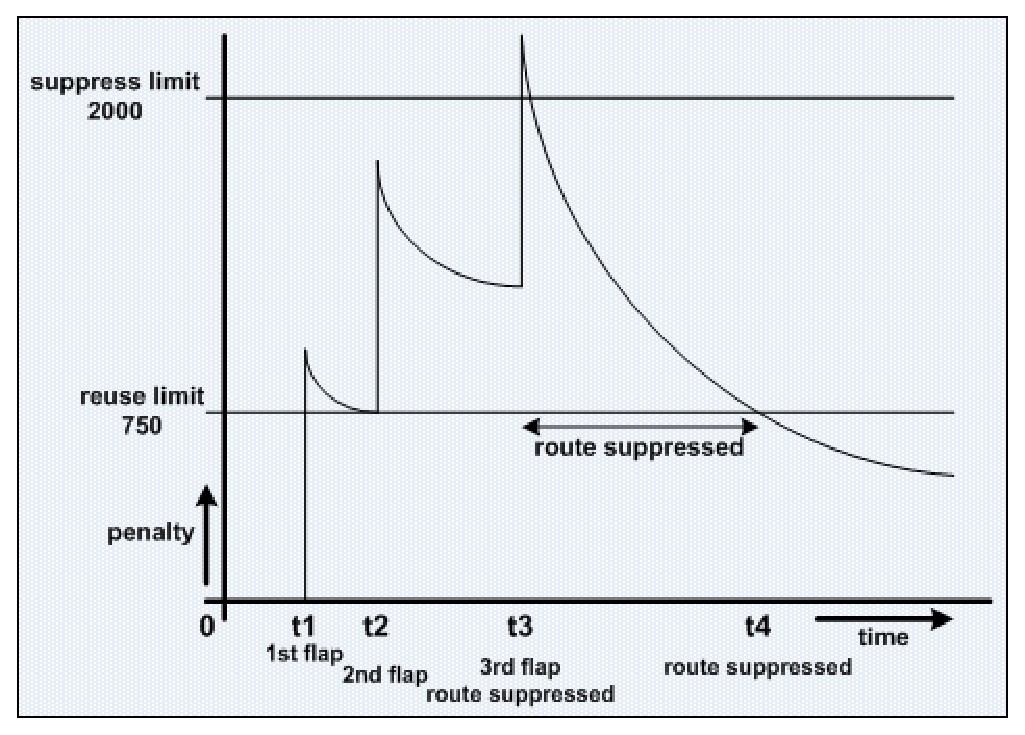
\includegraphics[scale=0.5]{route_damping} 
\par\end{center}
\caption{Typical evolution of the penalty assigned to a route.}
\label{fig_penalty}
\end{figure}

Penalty terms are re-computed at regular time intervals using timers.
Also, every time an update for a route is received, the penalty term
for that route is re-computed.

The RFC proposes several optimizations to decrease processing time,
at the cost of a slightly bigger memory footprint. \textit{E.g. reuse
lists} are used to avoid recomputing the figure of merit for all
routes : damped routes with similar penalty terms are grouped together
in a same reuse list. Penalty terms of the routes in a given reuse
list are then re-computed only when necessary.


\section{Implementation}

The implementation contains most of the data structure definitions
and functions needed for the route damping algorithm (RFC 2439).
As the RFC leaves little freedom regarding the implementation and the 
design of the data structures, our implementation closely matches the 
described specification.
The code, along with the list of commits, is publicly available on
{\tt\small \href{https://github.com/alexchap/Albatros-Project}
{https://github.com/alexchap/Albatros-Project}}.

Several parts of BIRD had to be modified for the implementation of route
damping. Some files used by the configuration parser had to be modified 
in order to correctly handle the parameters required by the RFC.
Also, we had to make similar modifications to the command line parser
so that suppressed routes could be listed using the \texttt{\small 
show dampened paths} command.
The \texttt{\small show protocols all} was also extended with a ``damped'' 
field, indicating the total number of currently damped routes.
Last but not least, we had to add hooks to BIRD's BGP implementation:
whenever a route is added or withdrawn, our code is executed.
Route damping is enabled at configure time by adding the 
{\tt\small -{}-enable-route-damping} switch.

\subsection{Data structures}

The data structures used by the implementation are very close to 
those described in the RFC (\S4.4, \textit{Run Time Data Structures}).
The most important of which are certainly {\tt\small damping\_config} and
{\tt\small damping\_info}.
Their definitions can be found in {\sl damping.h}.

{\tt\small damping\_config} groups all configurations parameters for a BGP peer.
This allows network administrators to have different sets of parameters for
different routes. {\it I.e} \texttt{\small damping\_config}s have a 
one-to-one relation to BIRD's \texttt{\small bgp\_proto}.
This structure contains all the parameters controlling the behaviour 
of the damping algorithm :
\texttt{\small reuse\_threshold}, \texttt{\small cut\_threshold}, 
\texttt{\small ceiling}, \texttt{\small tmax\_hold} and \texttt{\small half\_time}.
Additionally, it contains some information used to speedup the algorithm
(at the cost of a more important memory consumption) : both the decay
arrays and the reuse lists are contained here. The former speeds up the
computation of new figure of merits by pre-computing a predefined set
of (costly) exponentials and using them when figures of merit needs to 
be updated.
The latter limits the time of computation at every timer tick by 
grouping damped routes according to their penalty term.
Instead of being updated at every tick, a group of routes is updated 
once every $n$ ticks, where $n$ is the number of reuse lists.
Reuse lists are implemented using \texttt{\small slist}s, 
a doubly linked list implementation provided by BIRD.

BIRD's timer are used to regularly update the penalty terms of routes : 
every \texttt{\small bgp\_proto} structure contains a \texttt{\small 
reuse\_list\_timer}.
These timers are set up to call \texttt{\small damping\_reuse\_timer\_handler} 
at every tick.
This function is responsible for updating the penalty terms of 
damped routes and re-inserting damped routes into the routing table if their
penalty term is low enough.

The core of the damping algorithm lies with the \texttt{\small damping\_info} 
structure. The penalty term is stored in that structure, 
along with a timestamp indicating when the last update of the penalty term was.
Other pieces of information, such as the IP prefix of the route, reuse list pointers 
and route attributes (BIRD specific) are also included in \texttt{\small damping\_info}.
One such structure is allocated once a route starts to flap, and is de-allocated 
whenever the penalty term becomes ``small enough''.
There is a one-to-one mapping between routes (\texttt{\small rte} in BIRD) 
and \texttt{\small damping\_info}. This mapping was made possible by FIBs, 
an hash table implementation provided by BIRD's API. FIBs basically map IP 
prefixes to any other data structure, {\tt\small damping\_info}s in our case.

Last but not least, the fact that BIRD uses only one thread made our job much 
simpler as we didn't have to worry about concurrency.

\subsection{Configuration parameters}

Our extended version of BIRD gives network administrators a set of four 
parameters to control the behaviour of route damping.
In particular, {\tt\small cut\_threshold}, {\tt\small reuse\_threshold},
{\tt\small tmax\_hold} and {\tt\small half\_time} are all modifiable
from the configuration file.
Both {\tt\small tmax\_hold} (the maximum time a route can be kept damped, 
it defines the ceiling value) and {\tt\small half\_time} (the time taken by
a penalty term to diminish by half its value) are expressed in seconds.
Here is an example of configuration :

\begin{verbatim}
protocol bgp bgp_config {
  descriptionl "BGP daemon";
  debug all;

  # Specific config for BGP
  local as 65011;
  source address 10.10.10.11;
  multihop;
  next hop self;
  path metric 1;
 
  # Route damping configuration
  route damping;
  cut_threshold 2500;
  reuse_threshold 1000;
  tmax_hold 3000;
  half_time 900;
}
\end{verbatim}

The default parameters (hard coded in \textsl{damping.h}) are :

\begin{center}
\begin{tabular}{|l|c|}
\hline
\texttt{\small cut\_threshold} & 1500 \\
\hline
\texttt{\small cut\_threshold} & 750 \\
\hline
\texttt{\small half\_time} & 900 \\
\hline
\texttt{\small tmax\_hold} & 3000 \\
\hline
\end{tabular}
\end{center}

The {\tt\small route damping} parameters can be used to enable/disable
route damping for a particular neighbour. All the other parameters used by
the RFC (\textit{e.g.} decay arrays, scaling factor, ...) are either derived from
those four values or hard coded, as they should be hidden to the end-user.

BIRD uses Bison to parse the configuration files and we had to extend it 
to support the new set of keywords. Those parameters are passed to the 
{\tt\small damping\_config\_new} function, which allocates and initializes 
a new {\tt\small damping\_config} and computes the other parameters.
Finally, checks are made to ensure that the parameters are consistent with 
each other. \textit{E.g.} the \texttt{\small cut\_threshold} must be bigger
than \texttt{\small reuse\_threshold}, and damping should be enabled only for E-BGP.

\subsection{Detecting BGP Flapping}

Our implementation sticks to the RFC regarding route flapping detection.
Hooks were added in the BGP module of BIRD for that purpose.
Those hooks ensure that the {\tt\small damping\_add\_route} or 
{\tt\small damping\_remove\_route} functions are 
called when routes are advertised or withdrawn, respectively.

As those functions are similar to their equivalent in the RFC, only the relevant
implementation details are covered here.

When a route is removed for the first time, a new {\tt\small damping\_info} 
is allocated in a {\tt\small damping\_info\_fib}, and its penalty term is set to 
a default value. The penalty term of this route is updated as the route is re-advertised
and removed again. In particular, when the route is removed, its penalty term is
updated and then incremented by a default value : 1000, whereas its penalty term is just
updated when it is added. The penalty term is represented by a scaled integer,
so that only the right level of precision is kept during execution.
The main idea is that floating point operations are used when the figure of merit needs
to be updated, but the result is stored as an integer (thus saving memory space).
This usually results in an accidental loss of precision, except that in our case,
the decrease in precision is controlled so as not to crash the application. 
Penalty terms are all implicitly multiplied by 1000, implying that only three digits 
after the dot are kept.

{\tt\small damping\_info} are de-allocated when the penalty gets smaller than
{\tt\small reuse\_threshold} divided by two. The rationale being that when the penalty
term gets much smaller than the {\tt\small reuse\_threshold} index, keeping the 
{\tt\small damping\_info} structure with a small figure of merit is equivalent to de-allocating it 
(in the worst ---very unlikely --- case, it will only add the cost of re-allocating a 
new {\tt\small damping\_info} structure).

\section{Evaluation}

\subsection{Overview}

We used a topology of 27 routers in the NSL cluster to evaluate our implementation on a real scale basis.
This topology is composed of 10 Autonomous Systems and is displayed in figure \ref{fig_topo}
\begin{figure}
\begin{center}
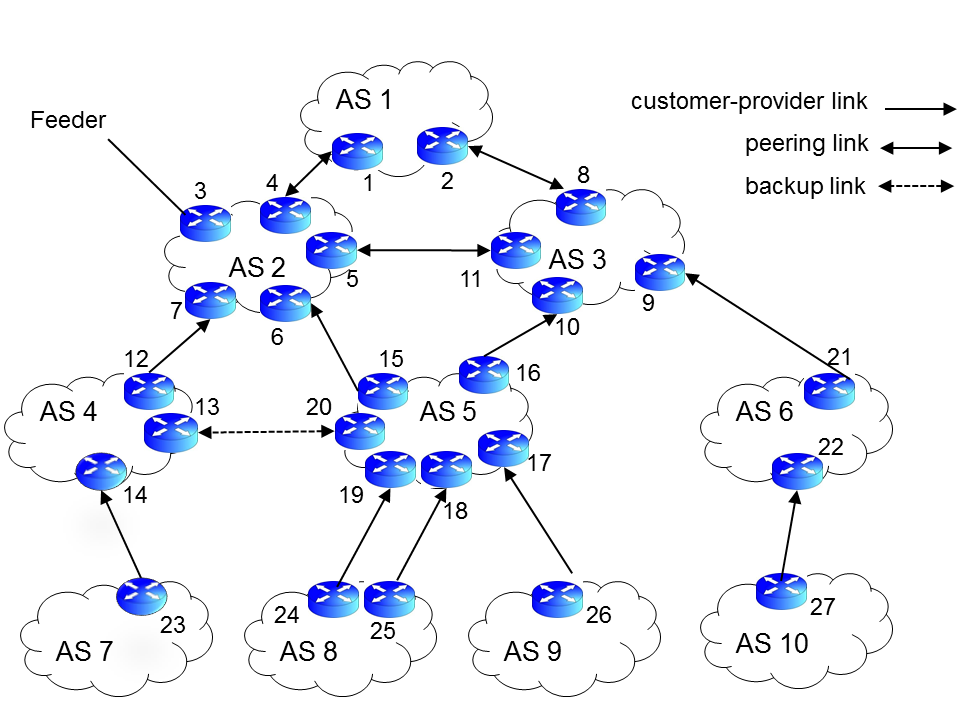
\includegraphics[scale=.3]{img/topology.png}
\end{center}
\caption{The topology used in our real scale experiments. \textit{Image courtesy of Marco Canini}}
\label{fig_topo}
\end{figure}

The experiment replays updates contained in an archive,
\textsl{updates.20100401.1729} (the archive comes from \cite{routeviews}).
This archive is composed of advertisements sent by 11 BGP routers and collected
over a period of time of 15 minutes.
All updates are sent to router 3 (\texttt{\small 10.0.0.3}), and then relayed into the network.
We carried out 3 experiments, with the same updates and different settings:

\begin{enumerate}
\item The first experiment was run with the original BIRD code, without route damping.
\item The second had route damping enabled and used the default parameters.
\item The third used a more aggressive \texttt{\small cut\_threshold} : 
it was lowered to 1000 (vs 1500 for the default setting).
\end{enumerate}

During these experiments, the number of updates and withdrawals were collected every 10 seconds 
(\textit{i.e.} we collected the total number of update/withdrawals received at every router).
The number of dampened routes was also collected, for the settings with route damping enabled.
The number of updates/withdrawals cumulates over time, whereas the number of dampened routes is immediate.
In the following subsections, the analysis of thoses measurements demonstrates the effectiveness
of route flap damping in the above-mentioned network.

\subsection{Evolution of dampened paths}

The evolution of dampened paths is shown on figure \ref{fig_dampenedpaths}: about 120 routes
are damped when reaching the end of the updates period.
The trend is similar for both experiments 2 and 3.
This is an expected result, as the exact same updates are sent in both cases.
We note however that more routes are damped with the more aggressive \texttt{\small reuse\_threshold} of experiment 3.
The number of damped routes grows with time.
Had we waited more time without sending any new updates, the curve would have sunk to eventually reach zero, as the penalty 
of each route would have decayed below \texttt{\small reuse\_threshold}.

\begin{figure}
\begin{center}
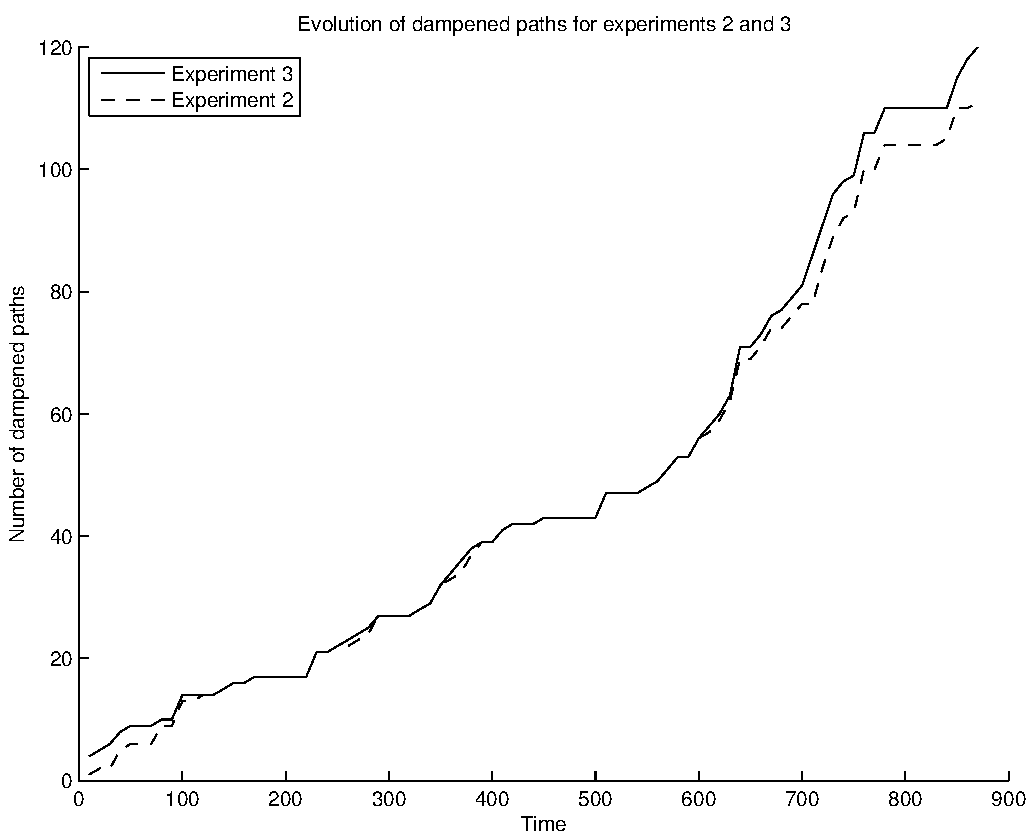
\includegraphics[scale=.5]{img/dampened_paths.pdf}
\end{center}
\caption{Evolution of \textbf{dampened paths} for experiments 2 and 3.}
\label{fig_dampenedpaths}
\end{figure}

\subsection{Number of route updates}

While it is interesting to see the evolution of the dampened paths, it is much more relevant 
to know how many updates were blocked, as limiting irrelevant traffic is precisely the aim of
the RFC. Figure \ref{fig_exp1_updates} shows the number of updates in experiment 1, aggregated 
per AS. Note that the total is rather big, reaching approximately 350 000 updates after only 
15 minutes of updates. 

Figure \ref{fig_diff_updates} represents the number of updates blocked by the damping algorithm. 
It's the number of updates in experiment 1 minus the number of updates in experiment 3. The 
total is quite representative of the benefits of BGP route flap damping: about 9000 updates 
could be avoided in the whole network. Even though it only accounts for a 2\% decrease 
in the total number of updates exchanged, the benefit would be clear in a real life scenario, 
when much more traffic and many more routers are involved.

\begin{figure}
\begin{center}
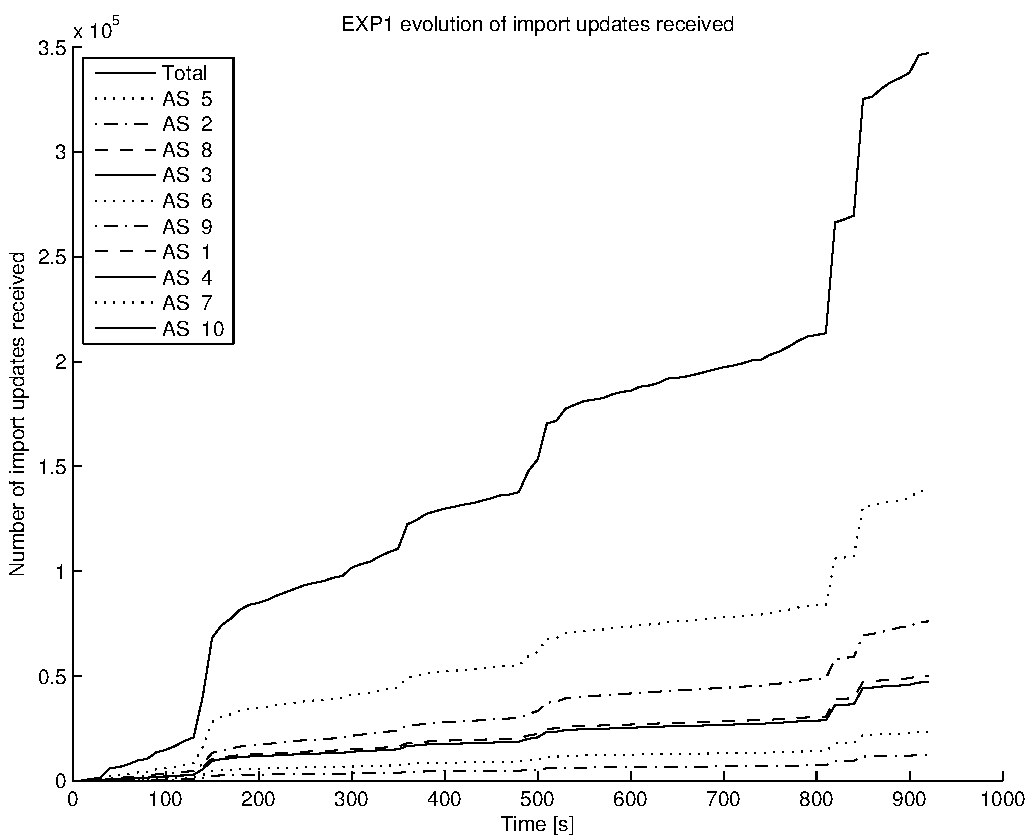
\includegraphics[scale=.5]{img/exp1_updates.pdf}
\end{center}
\caption{Evolution of \textbf{import updates} when damping is not activated.}
\label{fig_exp1_updates}
\end{figure}

\begin{figure}
\begin{center}
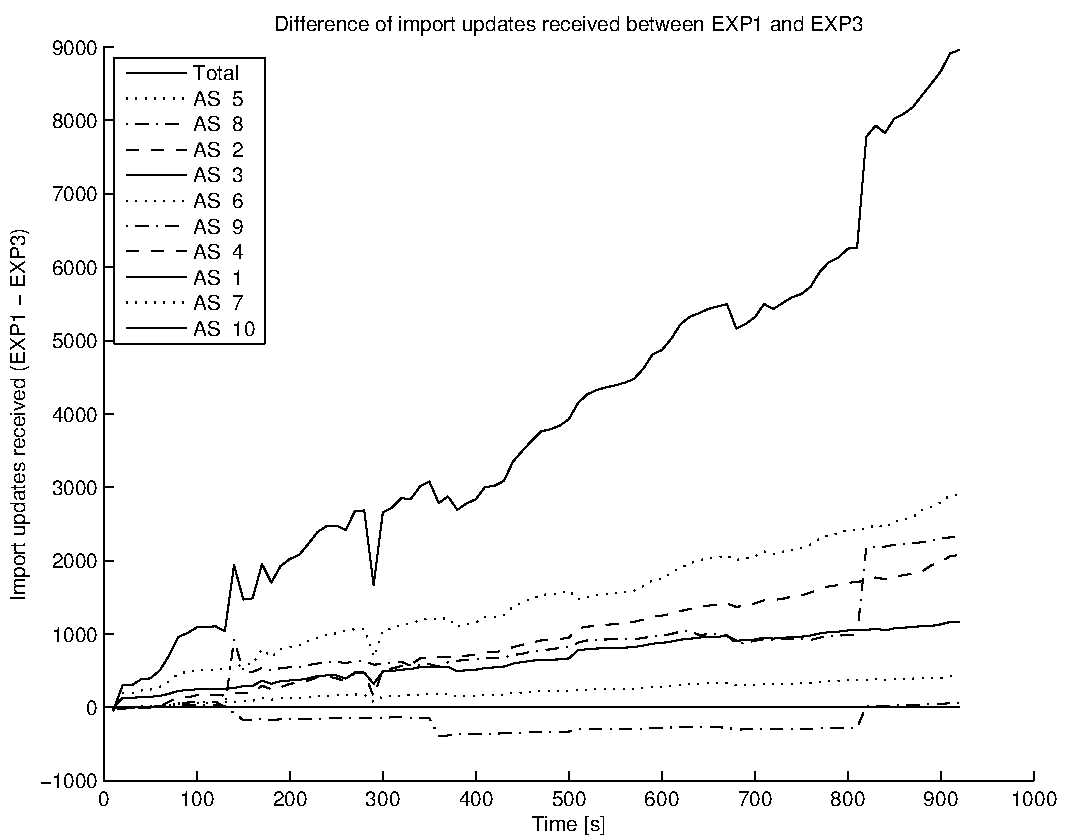
\includegraphics[scale=.5]{img/diff_exp1_exp3_updates.pdf}
\end{center}
\caption{Number of \textbf{blocked updates} in experiment 3.}
\label{fig_diff_updates}
\end{figure}

\subsection{Number of withdrawals}

Similarly, we measured the number of withdrawals per AS for all experiments. 
Figure \ref{fig_exp1_withdraws} shows the evolution of withdrawal messages when damping was not enabled, whereas figure \ref{fig_diff_withdraws}
shows the number of withdraws that were blocked during experiment 3. (The difference with respect to experiment 1).
About 650 withdraw messages were blocked after 15 minutes, which is approximately 10\% of the total number of withdraws received. The ratio is clearly 
better than for import updates in the previous subsection. The whole network gains in stability by receiving less withdrawals.

\begin{figure}
\begin{center}
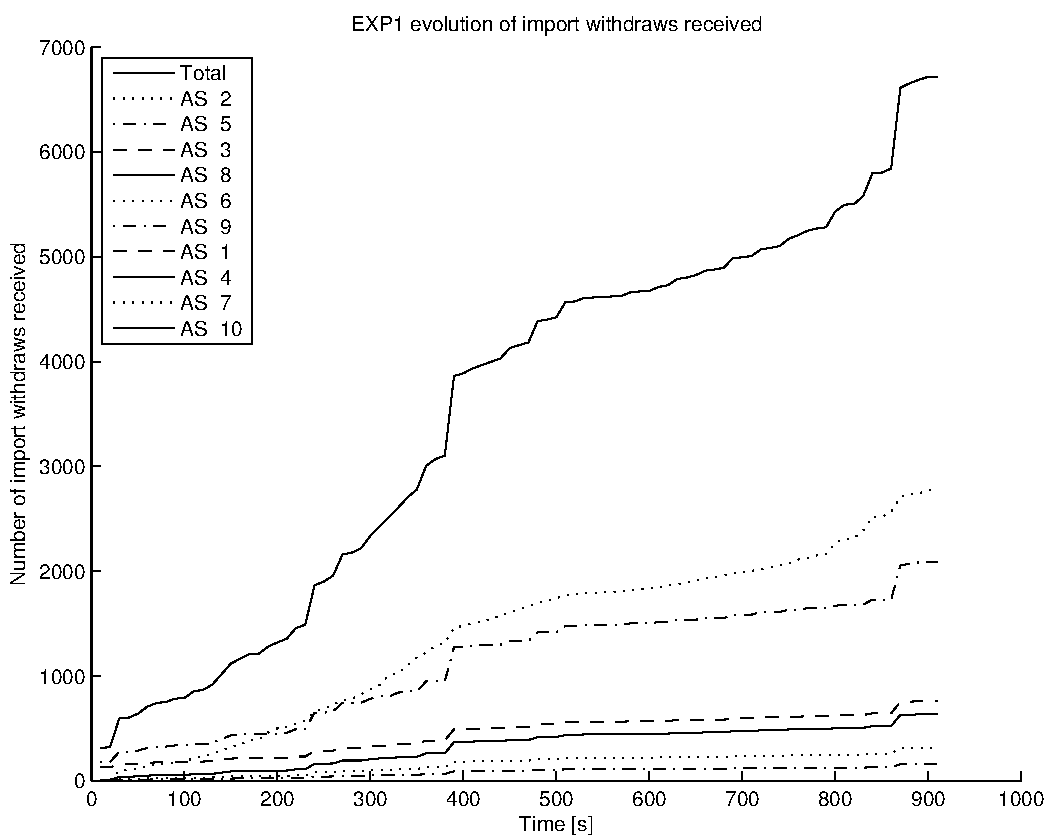
\includegraphics[scale=.5]{img/exp1_withdraws.pdf}
\end{center}
\caption{Evolution of \textbf{import withdraws} when damping is not activated.}
\label{fig_exp1_withdraws}
\end{figure}

\begin{figure}
\begin{center}
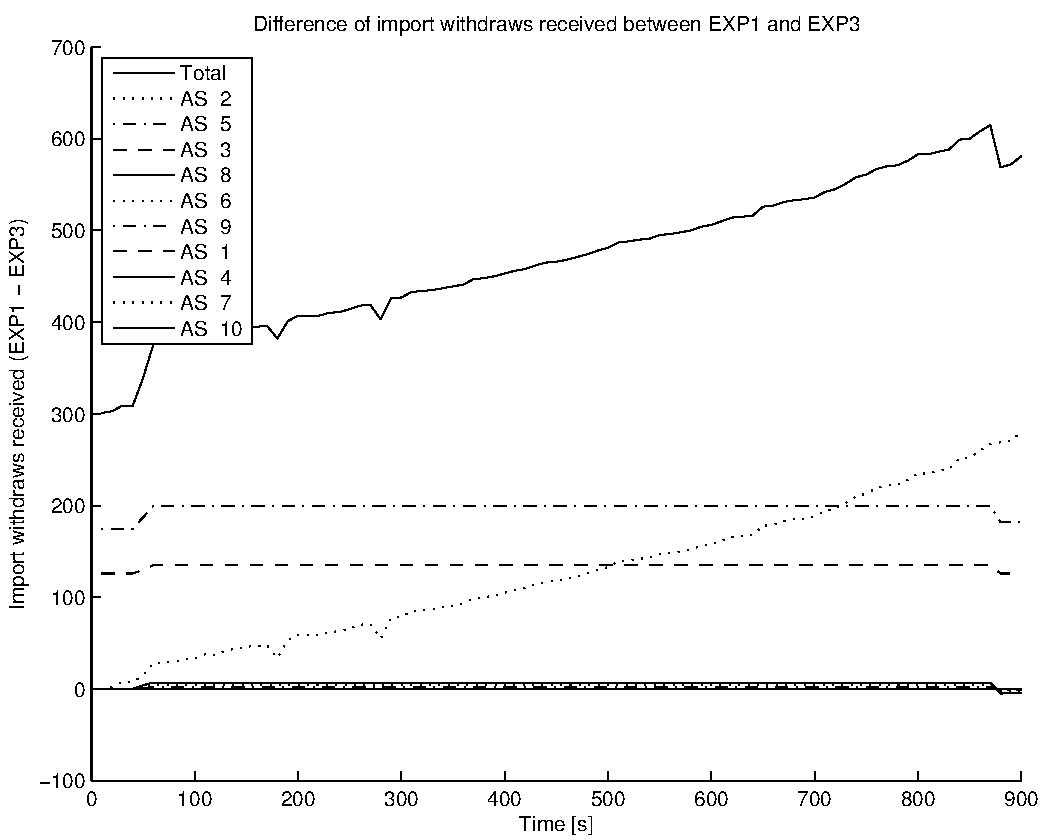
\includegraphics[scale=.5]{img/diff_exp1_exp3_withdraws.pdf}
\end{center}
\caption{Number of \textbf{blocked withdraws} in experiment 3}
\label{fig_diff_withdraws}
\end{figure}

\section{Conclusion}

Implementing one RFC for a routing software was not trivial. We managed to do it for the Bird routing project 
in a couple of weeks; the well-written coder's doc\cite{codersdoc} really helped us for this project.
Evaluation has been carried out on a small real-scale basis, with a network of 10 AS's and 27 routers. 
The measurements and corresponding analysis have shown that a ``simple'' method (around 1000 lines of C code) 
like that presented in RFC 2439 can significantly improve the overall health of a network.
It not only reduces the traffic, but can also help BGP converge by preventing unwanted routing traffic from 
spreading to the whole network.

\subsection{Future work}

Several extensions proposed in the RFC still need to be implemented.
For instance, the RFC suggests that a network administrator may want to have different behaviors for routes that 
are reachable or not. Alternate paths could also have been considered, before damping a route.

Initially, we also wanted to improve the algorithm of the RFC with a state-of-the-art extension, but understanding 
BIRD's code without prior experience took us more time than expected. We eventually ran
out of time and could barely finish the testing phase.
What's more, the Ipv6 version of route damping has not been implemented, but it should be quite easy to extend the current code.
Finally, it would have been really interesting to test route damping on a real internet, with more updates
than the 15 minutes dumps that have been replayed.

\section*{Acknowledgment}
We would like to thank the staff of the NSL @ EPFL, who let us carry out the experiments on powerful machines. 
A special thanks also to Marco Canini who helped us understanding how we could replay updates with the mdfmt tool.

\begin{thebibliography}{6}

\bibitem[1]{rfc2439}The RFC 2439, BGP Route Flap Damping, \href{http://www.ietf.org/rfc/rfc2439.txt}{http://www.ietf.org/rfc/rfc2439.txt}

\bibitem[2]{ripe recommendations} RIPE Recommendations On Route-flap
Damping, \href{http://www.ripe.net/ripe/docs/ripe-378}{http://www.ripe.net/ripe/docs/ripe-378}

\bibitem[3]{bird}Bird Routing Project, \href{http://bird.network.cz}{http://bird.network.cz}

\bibitem[4]{repository}Our publicly available repository, \href{https://github.com/alexchap/Albatros-Project}{https://github.com/alexchap/Albatros-Project}

\bibitem[5]{damping-pic}itcertnotes, \href{www.itcertnotes.com}{http://www.itcertnotes.com}

\bibitem[6]{routeviews}\href{http://routeviews.org}{http://routeviews.org} 

\bibitem[7]{codersdoc}\href{http://bird.network.cz/?get\_doc\&f=prog.html}{http://bird.network.cz/?get\_doc\&f=prog.html}

\end{thebibliography}

\end{document}
